\section{问题四 多区域算-储-电协同优化}

\subsection{模型与方法}

前三问已经解决了单区域任务调度、跨区域迁移还有储能时移的问题。问题四要求建立多区域算—储—电协同优化模型，统一考虑任务迁移、电价、碳排放、可用新能源、储能、区域购售电边界、网络时延及任务异构性。在系统运行成本、碳排放、网络时延、服务质量、新能源利用率和区域峰值净购电六项指标之间进行权衡，同时比较不同碳约束、电价与新能源下的场景。本问同时兼顾算力分配、时间调度和储能购售电之间的协同。对于多目标优化，采用主要目标法，以成本最小化为单一目标，将碳排放以$\varepsilon$约束嵌入。其余指标作事后评价，避免在高维空间直接求解Pareto前沿的不可行性。

我们在处理数据时发现，全耦合模型面临根本求解障碍。若把这50000个任务在2400时段上的开工决策全部作为0-1变量，则仅时间维度就会产生约3660万个候选变量。外加储能、购售电与消纳连续变量，其体量将远超HiGHS求解能力。但只约束截止时间与容量，又只能给出目的地分配，无法纳入电价感知的时移和新能源逐时匹配。因此我们借鉴国家对核能不参与调峰的政策，制定基荷预填策略。为了实现这一策略，我们将模型解耦为两层。层1以容量感知贪心确定目的地，通过新能源基荷预填预先固定大部分延迟容忍任务，使其移出层2的变量空间。层2为每区剩余的自由任务以及储能、购售电、消纳环节建立0-1 MILP，独立求解。变量空间从36.6M压至223个候选0-1变量，压缩约$1\times10^5$倍，以少量精度损失换取可解性。

\medskip\noindent\textbf{层 1：任务分配与新能源基荷预填。}六区域之间没有跨区电力潮流（赛题说明7），算力与电力只能借任务迁移间接耦合，目的地分配因此仍是第一层要解决的事。分配沿用问题二的容量感知贪心，对每项任务$j$，在时延可达集合$\mathcal{M}_j$内按$\text{PUE}_r\cdot\bar{\text{Price}}_r$升序，优先放进算力载荷未满的目的地；若候选区都逼近$\text{Cap}_r\cdot2400$的90\%阈值，则退而选择平均负载率最低的区域兜底。

分配完成后进入基荷预填。新能源出力逐时波动，若把各小时的可用量直接交给优化器，解会过于敏感；不如先画一条保守的出力基线。基线取各区域可用新能源的25\%分位，即$\text{Baseload}_r=Q_{25}(\text{Avail}_{r,t})=588\;\text{MW}$。这条线保证75\%的时段实际出力不低于它，只能算确定性的电量参考信号。优化器围绕它安排其余负载，天然获得低风险的调度下限。基线单位是功率（MW），要落到算力侧还需按PUE折算、扣掉不可调的NonAI负载，最终得到AI任务可占用的逐时配额
\begin{equation}
  \text{Quota}_{r,t} = \max\!\left(\frac{\text{Baseload}_r}{\text{PUE}_r} - \text{NonAI}_{r,t},\; 0\right),
\end{equation}
式中 $\text{Baseload}_r/\text{PUE}_r$ 为基荷功率对应的 IT 负荷上限，$\text{NonAI}_{r,t}$ 为不可调的固定负载，取下限 $0$ 保证配额非负。
随后我们把分配到区域$r$的延迟容忍任务按GPU-hour降序排列。在满足GPU容量与基荷配额约束的前提下，我们让占用资源大的任务优先调度。凡同时满足最早可行开工小时与GPU容量两个条件的任务，即被标记为基荷任务并退出层2。EDF失败的任务经第二轮重新分配，调往负载率最低且未满90\%容量的区域重试。仍然失败的50个任务进入层2显式优化。

实测50000个任务中33226个被基荷预填锁定，覆盖GPU-hour总量的95.3\%。E/F区是基荷主力，预填率分别为72.8\%与70.9\%。瓶颈在于GPU容量。D区则相反，配额充足但任务供给不足，预填率仅17.3\%。A/B区则经重新分配承接E/F溢出后才启用基荷。逐时核查显示，AI IT配额超过受限消纳上限$\text{Used}_{r,t}+\text{Rch}_{r,t}$的小时数占比为30\%--63\%；在这些超限小时上，六区域配额值的中位数介于165与290 MW之间。这表明相当比例的时段基荷任务新能源电力供应不足，缺口需购电补足。故基荷应该视作提供确定性电量信号以压缩变量的手段，其价值由Clean-test次优性与求解时间体现，不表述为碳减排主要来源。

\medskip\noindent\textbf{层 2：每区域独立 0-1 MILP。}层2对每区域建立独立0-1 MILP，合并问题一调度框架与问题三储能框架。决策变量含非基荷自由任务的0-1开关$x_{j,h}\in\{0,1\}$（$h\in\mathcal{W}_j$候选窗口）及储能SOC $E_t$、充电$C^g_t/C^r_t$、放电$D_t$、购电$G_t$、售电$S_t$、直供$R_t$等连续非负变量。目标为每区域运行成本最小化，含结清段2400--2405结算：
\begin{equation}
  \min\; Z_r = \sum_{t=0}^{2405}\!\big(G_t\,\text{Price}_{r,t} - S_t\,\text{SellPrice}_{r,t}\big).
\end{equation}
约束共八条：
\begin{itemize}
\item[(C1)] 恰好开工一次：$\sum_{h\in\mathcal{W}_j}x_{j,h}=1$；
\item[(C2)] GPU容量：自由、基荷固定与实时固定之和不超过$\text{Cap}_r$，引入容量越限松弛变量$s_t\ge0$、惩罚系数$10^6$元/GPU-hour；
\item[(C3)] 功率平衡：$G_t+R_t+D_t=\text{AI\_IT}_t\cdot\text{PUE}_r+\text{NonAI}_t\cdot\text{PUE}_r+C^g_t+S_t$；
\item[(C4)] 受限消纳：$R_t+C^r_t\le\text{Used}_t+\text{Rch}_t$（与问题三同口径）；
\item[(C5)] SOC递推：$E_t=E_{t-1}+\eta_c(C^g_t+C^r_t)-D_t/\eta_d$，终端$E_{2406}\ge E^{\text{init}}$；
\item[(C6)] 设备边界：容量、充放功率、购售电上限；
\item[(C7)] 同时充放由效率$\eta_c\eta_d<1$经成本目标自动排除（实测为0小时）；
\item[(C8)] 碳排放$\varepsilon$约束：$\sum_{t=0}^{2399}G_t\,c_{r,t}\le10^3\,\varepsilon\,C^{\text{base}}_r$，主解$\varepsilon=1.00$。
\end{itemize}

C2容量越限松弛，主解有所越限。F区有1小时超容318.7 GPU-hour，约为该区容量的33\%，在主时域2400小时中占比仅0.04\%。原因出在层1按平均负载率阈值分配目的地，未逐时核对容量。更棘手的是，即便层2已把F区自由度压缩到只剩2个自由任务，也就是64个候选变量，基荷预填与实时任务叠加后依然超限，说明仅靠选时没法消化这一缺口。求解器最终选择支付松弛惩罚，任务不做调整，故报告的成本指标不含惩罚项。

关于碳基准与$\varepsilon$约束的取值方式。主解$\varepsilon=1.00$的约束取值设为问题四自身无碳约束解的碳排放量。因为问题四负荷与问题三Baseline不同，E区最小固定负荷购电碳排放121.2 kt，已超问题三的84.6 kt。继续沿用问题三的基准将导致主解无可行解。若模型无碳约束解，即取$\varepsilon=1.00$不额外施加约束。因为波动会改变消纳能力、推动碳排放整体位移，所以新能源$\pm20\%$场景以模型无碳约束解重算取值；电价$\times1.5$场景则不重算，因为电价不影响碳排放，于是直接沿用基准场景取值。

\medskip\noindent\textbf{求解策略。}层 2 的每区域 MILP 经基荷预填后，0-1 变量维数大幅降低，最多 110 个，出现在 E 区。我们用开源的 HiGHS MILP 求解器求解。完整求解流程分为两个阶段。阶段 1 为层 1 分配与基荷预填，耗时 18.1 s。阶段 2 为层 2 六区 MILP，合计耗时 1.1 s，逐区 0.1--0.3 s。单场景完整求解约 19 s。主解 $\varepsilon=1.00$ 六区域全部求得全局最优。回带做自洽性检验全部通过，同刻充放为 0，SOC 终端合规，功率平衡残差约 $1\times10^{-13}$。

\subsection{结果与场景分析}

\medskip\noindent\textbf{主解六指标。}主解的六项全局指标为运行成本\textbf{2166.64 M 元}、碳排放\textbf{1960.78 kt}、区域峰值净购电功率\textbf{550.0 MW}、新能源利用率\textbf{20.83\%}、GPU-hour加权平均时延\textbf{28.07 ms}、服务质量按时完成率\textbf{100\%}。分区域结果见表~\ref{tab:sub4-main}，六区特色明显，A、B、C 是高电价高负荷区，成本512--578 M 元，实时任务全部落在这一组，只额外承接少量重新分配的基荷任务；D 区作为低成本算力中心，成本142.37 M 元、利用率24.8\%，预填率仅17.3\%。D区预填率低的原因在于本地任务供给不足。E、F 区是基荷电量主力，预填率分别达72.8\%与70.9\%，延迟容忍任务大量在此落地，靠的正是低价低碳的区位优势。

\begin{table}[H]
\centering
\footnotesize
\caption{问题四主解六区域明细（$\varepsilon=1.00$，主时域 0--2399；$n_x$ 为区域候选 0-1 变量数，即自由任务窗口长度之和）}
\label{tab:sub4-main}
\begin{tabular}{lcccccc}
\toprule
区域 & 成本 (M元) & 碳排放 (kt) & 峰值 (MW) & 利用率 (\%) & $n_x$ & 角色 \\
\midrule
A & 578.28 & 547.08 & 550.0 & 8.5 & 0 & 实时为主，承接改投任务 \\
B & 530.06 & 487.95 & 520.0 & 10.0 & 0 & 实时为主，承接改投任务 \\
C & 512.91 & 460.19 & 510.0 & 11.8 & 0 & 实时为主（1.5万任务） \\
D & 142.37 & 186.37 & 510.0 & 24.8 & 49 & 算力中心，基荷 17.3\% \\
E & 188.36 & 124.45 & 370.0 & 36.0 & 110 & 基荷主力 72.8\% \\
F & 214.67 & 154.75 & 340.0 & 34.0 & 64 & 基荷主力 70.9\% \\
\midrule
\textbf{聚合} & \textbf{2166.64} & \textbf{1960.78} & \textbf{550.0} & \textbf{20.83} & 223 & \\
\bottomrule
\end{tabular}
\end{table}

六区域成本与碳排放分布见图~\ref{fig:sub4-region}（E/F区承担主要算力负荷），净购电与SOC的时序联动机理见图~\ref{fig:sub4-mechanism}。

\medskip\noindent\textbf{基线对比与成本归因。}为了看清主解的价值，我们先把它与两组无储能的贪心基线做六指标对照。B1 完全按 EDF 排程，不感知电价。B2 按电价贪心，为每个任务挑电价最低的开工小时。对照结果是主解成本 2166.64 M，比 B1 的 2253.57 M 低 86.93 M，降幅约 3.9\%；比 B2 的 2216.74 M 低 50.10 M，降幅约 2.3\%。两基线均有容量越限且未计越限惩罚，故上述降幅为近似值。主解与问题三储能解都包含储能环节，可比性更强。主解成本 2166.64 M 较问题三的 2213.35 M 低约 2.1\%，碳排放也由 2044.79 kt 降至 1960.78 kt，降幅约 4.1\%。

成本归因方面，我们分别关掉储能、关掉售电机制再重跑 MILP，比较成本差异。储能能量时移使成本抬升 137.71 M 元，F 区有 111 小时，购电量与储电量加和超过最大购电限制；售电机制仅省下 1.40 M 元；调度结构才为降低成本的主要贡献，省下 224.38 M 元。

再看碳排放。主解 1960.78\,kt 比 B1 的 1927.03\,kt 还高出 1.7\%。任务迁移重构了各区域的负荷比例，碳减排主要来自这里，基荷预填本身没有有效降低碳排放。此外，E、F 区承担了最多的基荷，碳排放比问题三高出 $+47\%$ 与 $+37\%$，正好印证这一点。预填只把开工时点提前，受限消纳下购电总量不变，它的价值在于给出可解方案、并加速求解。

\medskip\noindent\textbf{场景对比与敏感性。}
四组关键场景对比见表~\ref{tab:sub4-scenario}。碳约束压降场景下，$\varepsilon=0.95$仅D区可行（该行成本与碳排放为D区单区值），$\varepsilon=0.90$全区域无可行解。这验证了区域碳排放刚性。A/B/C区$\varepsilon_{\min}\approx0.99$、E/F区$\approx0.97$、D区0.9053，与问题三定性结论一致。峰谷价差$\times1.5$时，成本从2166.64线性升至2704.16\,M，碳排放不变（1960.79\,kt），电价只改变成本水平不改变调度结构。新能源$\pm20\%$时，成本近似对称变动（$-206.65$与$+217.30$\,M），碳排放随之同向变化（1793.03与2128.59\,kt），符合线性预期。

\begin{table}[H]
\centering
\footnotesize
\caption{问题四场景对比（$\varepsilon$ 约束取值按声明规则重算）}
\label{tab:sub4-scenario}
\begin{tabular}{lccccc}
\toprule
场景 & 成本 (M元) & 碳排放 (kt) & 峰值 (MW) & 利用率 (\%) & 可行性 \\
\midrule
S0 基准 $\varepsilon{=}1.00$ & 2166.64 & 1960.78 & 550.0 & 20.83 & 全可行 \\
$\varepsilon{=}0.95$ & 143.54$^{\dagger}$ & 177.05$^{\dagger}$ & 510.0$^{\dagger}$ & 24.8$^{\dagger}$ & 仅 D 可行 \\
峰谷价差 $\times1.5$ & 2704.16 & 1960.79 & 550.0 & 20.83 & 全可行 \\
新能源 $+20\%$ & 1959.99 & 1793.03 & 550.0 & 20.83 & 全可行 \\
新能源 $-20\%$ & 2383.94 & 2128.59 & 550.0 & 20.83 & 全可行 \\
\bottomrule
\end{tabular}
\par\smallskip\footnotesize
$^{\dagger}$ 该行数据为 D 区单区值，非全局聚合（其余五区无可行解）。
\end{table}

场景成本与碳排放联动见图~\ref{fig:sub4-scenario}。峰谷价差与新能源波动的灵敏度结果见§8.4。

\medskip\noindent\textbf{基荷策略检验与 Clean-test。}
为量化EDF预填相对MILP全局选时的次优性，我们设计了Clean-test配对实验。该实验设三档基荷比例阈值$\theta\in\{0.7,0.5,0.3\}$，EDF预填至$\theta\times$区域GPU容量即停止，其余的任务交层2 MILP全窗口选时。禁止重新分配，释放任务留在原区。每区按GPU-hour（后文简称GH）分层抽样40个任务构成配对样本，分别以EDF固定方案与MILP自由选时方案求解，成本差按GH比例放大。结果显示，预填比例从81.5\%（$\theta=0.7$）降到62.6\%（$\theta=0.5$）、43.6\%（$\theta=0.3$）时，MILP选时收益从$+0.88\%$升到$+2.10\%$、$+2.92\%$。$\theta$越低释放任务越多、收益越大，方向单调。主解预填95.3\% GH，其EDF次优性由单调性推断为\textbf{$<0.88\%$}（$\theta=0.7$档为正常高估，两者释放任务集合不同；主解仅4.7\% GH交MILP精细优化，实际次优性远小于此值）。

对不可解的$\theta=0$全任务MILP，我们采用大邻域搜索LNS作为验证手段。该搜索以B2电价贪心解为起点，每轮GH分层抽样$K=300$个任务构建子MILP，邻域窗口截断为$W=168$小时（保留当前选时以保证单调改进），每区50轮。LNS终值2139.60\,M（$\theta=0.3$结构、禁止重新分配），B2到LNS增量0.68\%，EDF到LNS全程约2.3\%，达Clean-test上界2.92\%的约78\%。需要说明，LNS终值含容量越限，E/F区各约31k GH松弛，且禁止重新分配使任务锁定在原区。但由于无法将LNS 与主解的成本计算规则对应，所以不可直接比较。收敛曲线（图~\ref{fig:sub4-lns}）末段斜率趋平（$-0.009$与$-0.014$\,M/轮），收敛成立。LNS增益低于Clean-test的主因是$W=168$\,h截断排除了把任务改晚到低价时段的搜索方向（恰是Clean-test大增益来源），故LNS增量是截断窗口下的保守下界。

\begin{figure}[H]
\centering
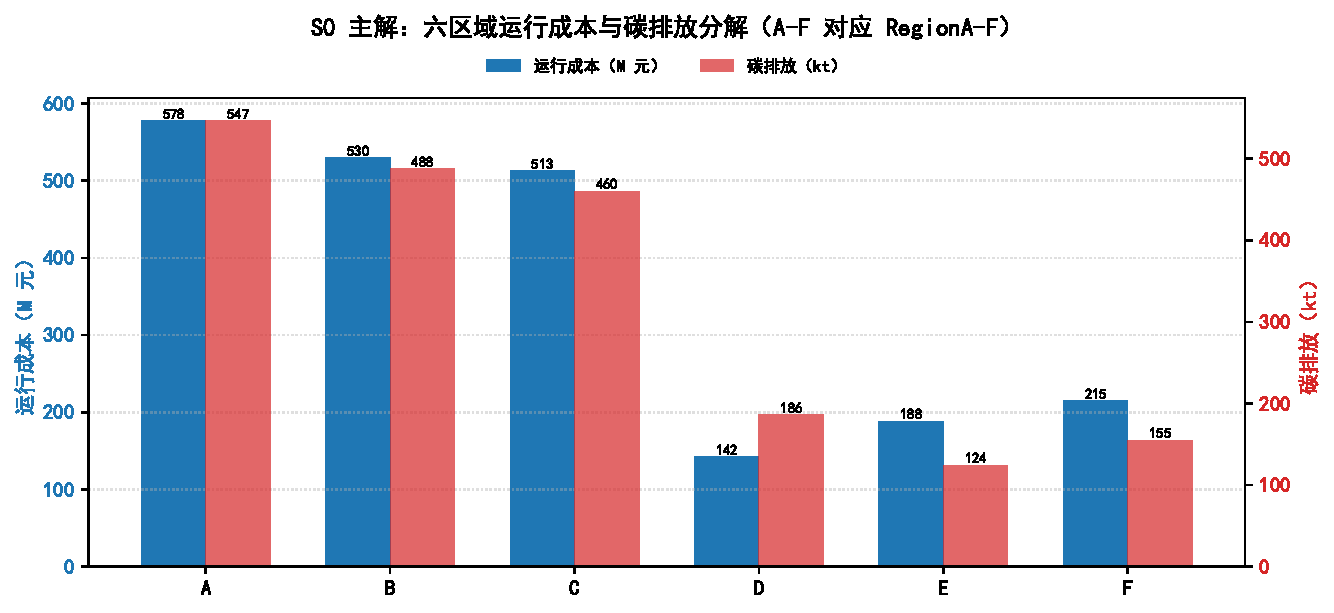
\includegraphics[width=0.95\textwidth]{../../outputs/figures/sub4-region-cost-carbon.pdf}
\caption{六区域成本与碳排放分布（A/B/C 高电价高负荷，E/F 低价低碳）（AI 辅助生成）}
\label{fig:sub4-region}
\end{figure}

\begin{figure}[H]
\centering
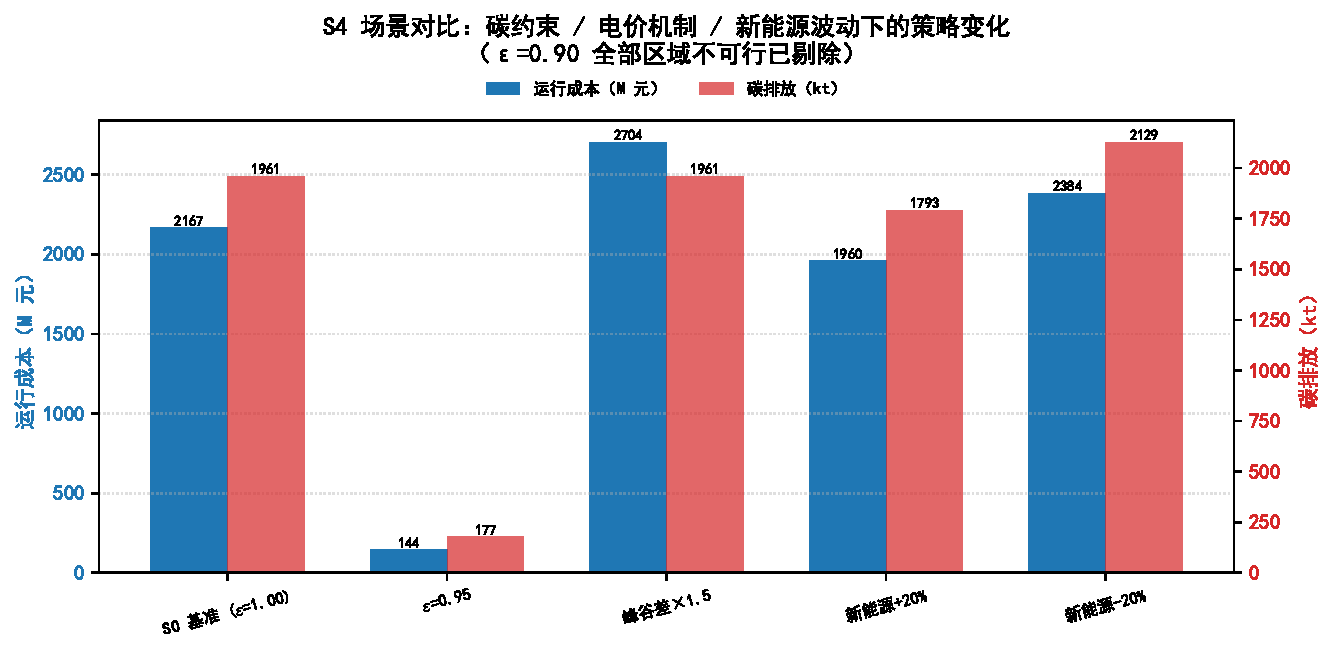
\includegraphics[width=0.95\textwidth]{../../outputs/figures/sub4-scenario-compare.pdf}
\caption{场景对比双轴柱状（成本/碳排放，部分可行标注）（AI 辅助生成）}
\label{fig:sub4-scenario}
\end{figure}

\begin{figure}[H]
\centering
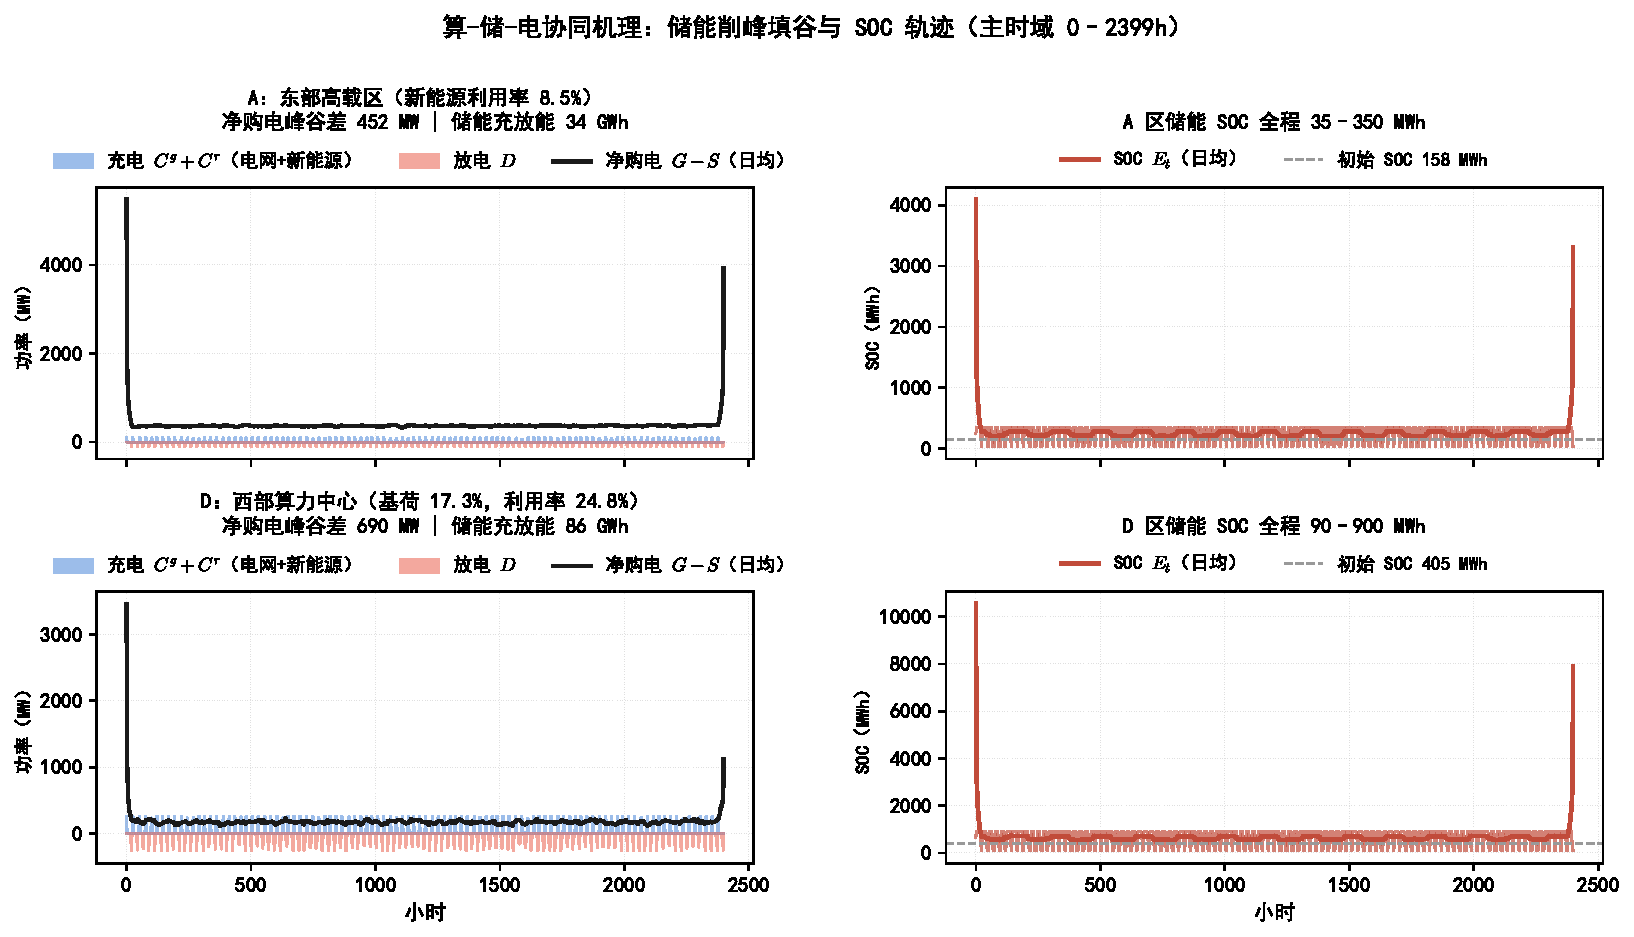
\includegraphics[width=0.95\textwidth]{../../outputs/figures/sub4-mechanism-net.pdf}
\caption{算-储-电机理，A（东部高负荷）与 D（算力中心）净购电 + SOC 时序（AI 辅助生成）}
\label{fig:sub4-mechanism}
\end{figure}

\begin{figure}[H]
\centering
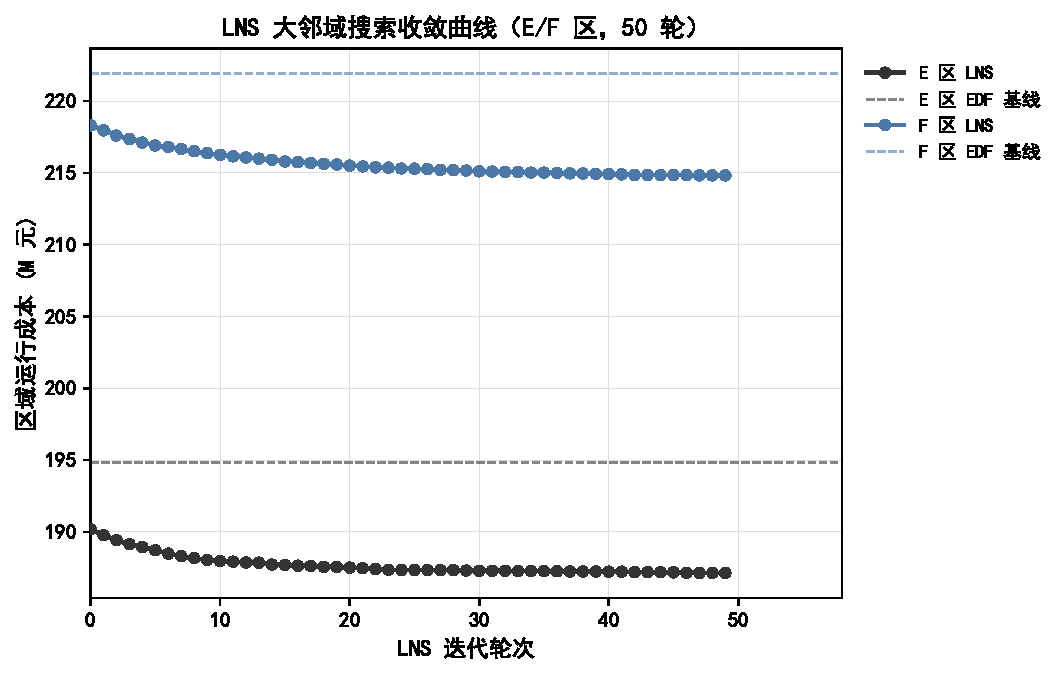
\includegraphics[width=0.95\textwidth]{../../outputs/figures/sub4-lns-convergence.pdf}
\caption{LNS 收敛曲线（E/F 区 50 轮，EDF 基线虚线对照 + B2 起点/终值标注）（AI 辅助生成）}
\label{fig:sub4-lns}
\end{figure}

综上，问题四的半耦合两层分解在可解性与精度间取得工程可接受平衡。主解以约19\,s/场景给出全局可行的六指标方案，基荷预填的EDF次优性经Clean-test量化控制在$<0.88\%$，LNS则验证了极端情形下的分解路径；碳约束的区域刚性、电价与新能源波动的线性响应共同刻画了模型特征与边界。
